```latex
\documentclass[12pt]{article}

%===========================================================
% PACKAGES
%===========================================================

\usepackage{graphicx}
\graphicspath{{./figures/}}

\usepackage{caption}
\usepackage[font=scriptsize]{subcaption}
\captionsetup[figure]{labelsep=none}
\captionsetup[table]{labelsep=none}

\usepackage{amssymb}
\usepackage{amsmath}
\usepackage{array}
\usepackage{booktabs}
\usepackage{float}
\usepackage{pdflscape}
\usepackage{adjustbox}
\usepackage{threeparttable}
\usepackage[margin=1in]{geometry}

\floatstyle{plaintop}
\restylefloat{table}


%===========================================================
% DOCUMENT
%===========================================================

\begin{document}


%=====================================================================
% FIGURE 1
%=====================================================================

\begin{figure}[H]
    \centering

    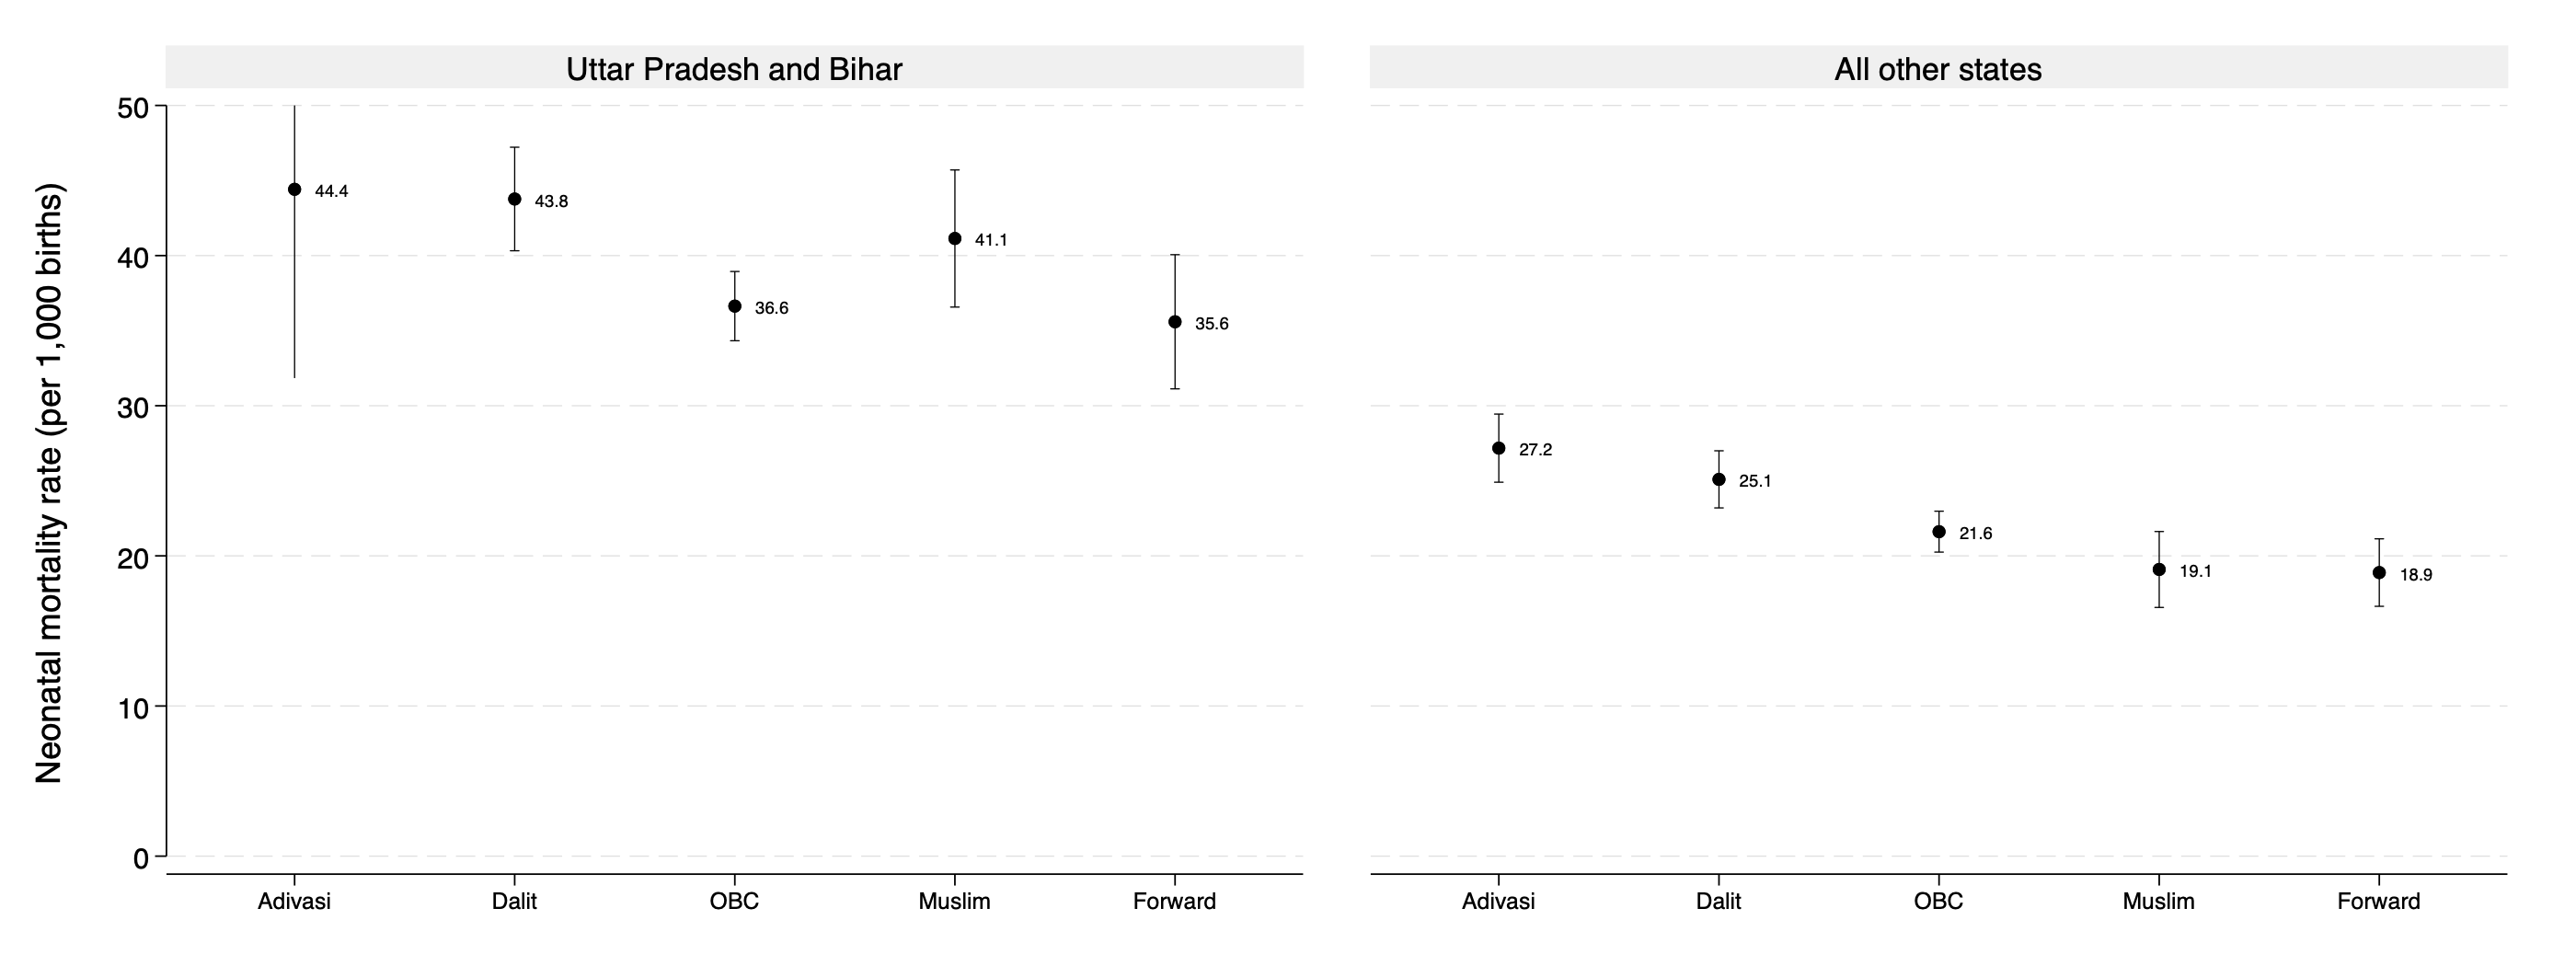
\includegraphics[
        width=\textwidth
    ]{figures/figure1 overall nnm UP Bihar other states NFHS4,5.png}

    \caption{
        : Disparities in neonatal mortality for all rural births
    }
    \label{fig:fig1}

    \vspace{0.4em}

    \begin{minipage}{0.96\textwidth}
        \scriptsize
        \textit{Notes:}
        The sample consists of rural births in NFHS-4 and NFHS-5.
        Adivasi includes Scheduled Tribe mothers, Dalit includes Scheduled
        Caste mothers, Muslim includes Muslim mothers who are not Scheduled
        Caste or Scheduled Tribe, OBC includes Hindu or Sikh mothers in
        Other Backward Classes, and forward caste Hindu includes Hindu
        mothers who are not Scheduled Caste, Scheduled Tribe, or OBC.
    \end{minipage}

\end{figure}


\clearpage


%=====================================================================
% FIGURE 2
%=====================================================================

\begin{figure}[H]
    \centering

    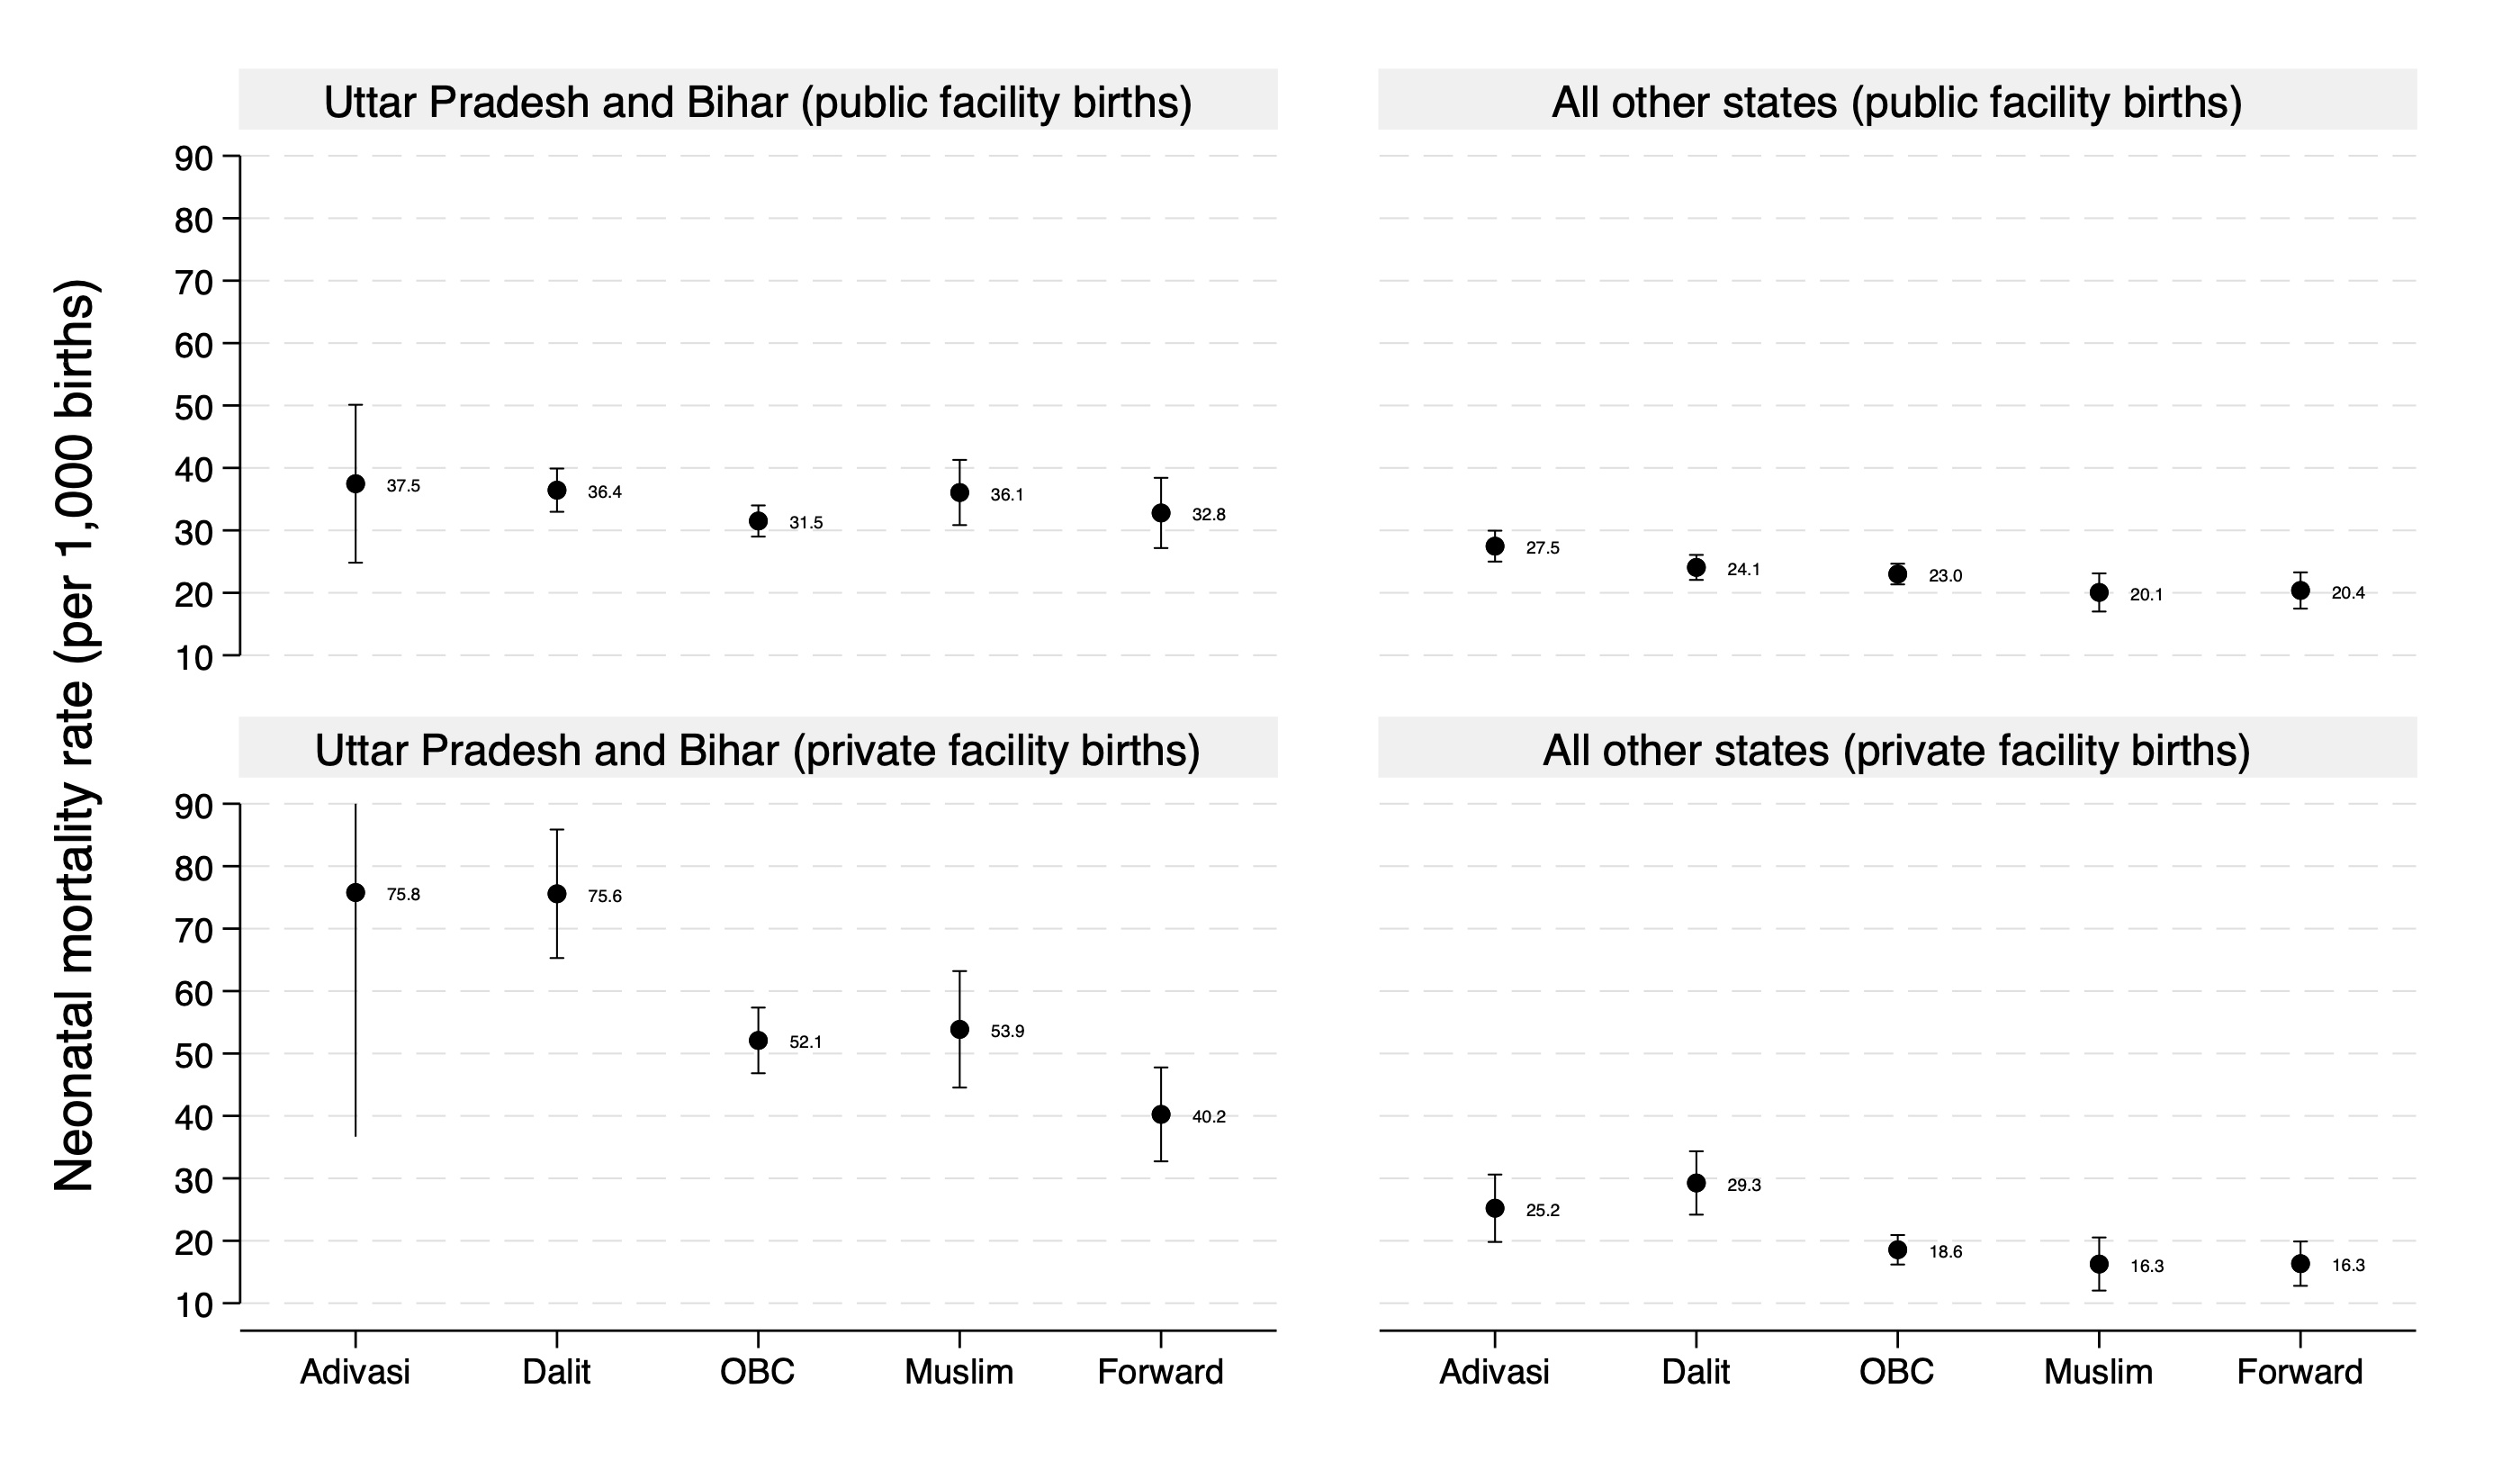
\includegraphics[
        width=\textwidth
    ]{figures/figure2 nnm public private UP Bihar NFHS4,5.png}

    \caption{
        : Disparities in neonatal mortality are larger among private
        facility births in Uttar Pradesh and Bihar
    }
    \label{fig:fig2}

    \vspace{0.4em}

    \begin{minipage}{0.96\textwidth}
        \scriptsize
        \textit{Notes:}
        The sample consists of rural births in NFHS-4 and NFHS-5.
        Adivasi includes Scheduled Tribe mothers, Dalit includes Scheduled
        Caste mothers, Muslim includes Muslim mothers who are not Scheduled
        Caste or Scheduled Tribe, OBC includes Hindu or Sikh mothers in
        Other Backward Classes, and forward caste Hindu includes Hindu
        mothers who are not Scheduled Caste, Scheduled Tribe, or OBC.
    \end{minipage}

\end{figure}


\clearpage


%=====================================================================
% TABLE 1
%=====================================================================

\begin{landscape}

\renewcommand{\arraystretch}{1.2}
\setlength{\tabcolsep}{9pt}

\begin{table}[H]
    \centering

    \caption{
        : Private facility births are socioeconomically advantaged across
        social groups, while differences in maternal and birth risk are mixed
    }
    \label{tab:private_public_characteristics}

    \vspace{0.4em}

    \begin{threeparttable}

        \begin{adjustbox}{max width=\linewidth}
            \scriptsize
            \begin{tabular}{l*{5}{c}@{\hspace{1.4em}}c@{\hspace{1.4em}}*{5}{c}}
\toprule
& \multicolumn{5}{c}{Uttar Pradesh and Bihar} & & \multicolumn{5}{c}{All other states} \\
\cmidrule(lr){2-6} \cmidrule(lr){8-12}
\addlinespace[0.25em]
& \tiny Adivasi & \tiny Dalit & \tiny OBC & \tiny Forward & \tiny Muslim & & \tiny Adivasi & \tiny Dalit & \tiny OBC & \tiny Forward & \tiny Muslim \\
\midrule
&&&&&&&&&&&\\
\textbf{Maternal and birth risk}&&&&&&&&&&&\\
\hspace*{2em}Mother under 20 at birth&-1.2&-0.5&0.3&-0.8&0.1&&1.0&-1.9***&-0.8*&-2.6***&-4.3***\\
\hspace*{2em}Male child&6.0*&2.1**&3.4***&3.1**&0.7&&2.4**&1.1&0.4&0.6&0.9\\
\hspace*{2em}Multiple birth&2.5&1.8***&1.3***&1.0*&1.2**&&0.6&1.5***&1.7***&1.3***&1.1**\\
\hspace*{2em}Prior neonatal death to mother&3.3*&2.0***&0.8***&0.4&0.2&&0.2&0.9***&0.2&-0.3&-0.1\\
\hspace*{2em}Projected maternal underweight&-10.8***&-8.4***&-7.7***&-8.4***&-9.5***&&-3.8***&-5.1***&-4.8***&-5.7***&-6.1***\\
\hspace*{2em}Birth order&-0.14&-0.34***&-0.34***&-0.37***&-0.39***&&-0.23***&-0.19***&-0.18***&-0.15***&-0.19***\\
&&&&&&&&&&&\\
\textbf{Pregnancy and delivery complications}&&&&&&&&&&&\\
\hspace*{2em}Breech presentation&1.8&1.6**&0.1&-0.4&0.4&&1.4&-0.7&0.9*&0.3&4.4***\\
\hspace*{2em}Prolonged labor&11.9***&7.2***&3.8***&1.7&2.3&&0.6&-4.5***&-3.9***&-2.7***&-4.8***\\
\hspace*{2em}Excessive bleeding&4.6&2.2*&-1.6**&-2.6*&-2.8*&&-2.1&-4.2***&-3.2***&-2.8***&-6.8***\\
\hspace*{2em}C-section birth&25.0***&29.3***&29.7***&34.4***&27.4***&&27.8***&32.0***&31.0***&28.6***&29.6***\\
&&&&&&&&&&&\\
\textbf{Socioeconomic characteristics}&&&&&&&&&&&\\
\hspace*{2em}Mother illiterate&-14.2***&-12.6***&-16.0***&-14.8***&-16.0***&&-18.5***&-9.7***&-10.1***&-9.7***&-13.3***\\
\hspace*{2em}Mean wealth quintile (1--5)&0.54***&0.54***&0.65***&0.73***&0.77***&&0.84***&0.63***&0.69***&0.79***&1.02***\\
&&&&&&&&&&&\\
\textbf{Care at birth}&&&&&&&&&&&\\
\hspace*{2em}Breastfeeding initiated within 1 hour&-3.6&-9.7***&-9.4***&-9.0***&-7.8***&&-8.7***&-7.8***&-7.8***&-7.5***&-1.4\\
\hspace*{2em}Skin-to-skin contact&-11.5**&-21.6***&-21.6***&-25.6***&-18.6***&&-11.5***&-8.1***&-6.2***&-7.9***&-1.8\\
&&&&&&&&&&&\\
\textbf{General}&&&&&&&&&&&\\
\hspace*{2em}Percent births in private facilities&18.1&18.7&24.9&37.6&28.5&&13.3&19.8&31.4&37.0&25.6\\
\hspace*{2em}Sample size&1,604&19,713&36,197&8,576&9,677&&54,587&42,212&66,819&29,223&23,134\\
\bottomrule
\end{tabular}

        \end{adjustbox}

        \vspace{0.5em}

        \begin{minipage}{0.92\linewidth}
            \scriptsize
            \textit{Notes:}
            With the exception of those under the ``General'' subheader,
            entries report differences between private and public facility
            births (private minus public) within each social group and region.
            Estimates are obtained from regressions of each characteristic on
            indicators for social group, private facility birth, and their
            interactions, estimated separately by region.

            Binary characteristics are reported in percentage points; other
            variables are reported in their original units.

            * $p<0.10$, ** $p<0.05$, *** $p<0.01$ indicate whether the
            private--public difference within a social group is statistically
            different from zero.

            $\dagger$ indicates that the private--public difference for that
            social group is statistically different from the corresponding
            difference among forward Hindu births at $p<0.05$.

            The sample consists of rural public and private facility births
            in NFHS-4 and NFHS-5 for which the variables used in the table
            are observed.
        \end{minipage}

    \end{threeparttable}

\end{table}

\setlength{\tabcolsep}{6pt}
\renewcommand{\arraystretch}{1}

\end{landscape}


\clearpage


%=====================================================================
% TABLE 2
%=====================================================================

\begin{landscape}

\renewcommand{\arraystretch}{0.7}
\setlength{\tabcolsep}{12pt}

\begin{table}[H]
    \centering

    \caption{
        : The larger private--public gap in neonatal mortality for
        disadvantaged social groups in Uttar Pradesh and Bihar is not
        accounted for by observed birth characteristics or local area
        differences
    }
    \label{tab:nnm_interactions}

    \vspace{0.4em}

    \begin{threeparttable}

        \begin{adjustbox}{max width=\textwidth}
            \scriptsize
            {
\def\sym#1{\ifmmode^{#1}\else\(^{#1}\)\fi}
\begin{tabular}{l*{6}{c}}
\toprule
            &\multicolumn{3}{c}{Uttar Pradesh and Bihar}                      &\multicolumn{3}{c}{All other states}                             \\\cmidrule(lr){2-4}\cmidrule(lr){5-7}
            &\multicolumn{1}{c}{(1)}&\multicolumn{1}{c}{(2)}&\multicolumn{1}{c}{(3)}&\multicolumn{1}{c}{(4)}&\multicolumn{1}{c}{(5)}&\multicolumn{1}{c}{(6)}\\
            &\multicolumn{1}{c}{No controls}&\multicolumn{1}{c}{Risk controls}&\multicolumn{1}{c}{+ Cluster FE}&\multicolumn{1}{c}{No controls}&\multicolumn{1}{c}{Risk controls}&\multicolumn{1}{c}{+ Cluster FE}\\
\midrule
Intercept (Forward public reference)&        24.5\sym{***}&        33.1\sym{***}&        26.6\sym{***}&        13.4\sym{***}&        14.6\sym{***}&        15.5\sym{***}\\
            &       (2.8)         &       (5.0)         &       (5.4)         &       (1.3)         &       (2.1)         &       (2.4)         \\
\addlinespace
Adivasi     &        -1.9         &        -7.9         &         1.7         &         5.3\sym{***}&         1.0         &         0.4         \\
            &       (5.9)         &       (5.8)         &       (6.1)         &       (1.5)         &       (1.6)         &       (2.3)         \\
\addlinespace
Dalit       &         3.5         &        -1.8         &         5.1         &         2.8\sym{*}  &         1.1         &         0.9         \\
            &       (3.2)         &       (3.3)         &       (4.1)         &       (1.5)         &       (1.4)         &       (1.9)         \\
\addlinespace
OBC         &        -0.1         &        -3.5         &         3.8         &         1.7         &         1.0         &        -1.5         \\
            &       (3.0)         &       (3.0)         &       (3.7)         &       (1.4)         &       (1.4)         &       (1.8)         \\
\addlinespace
Muslim      &         2.1         &        -3.0         &        -3.5         &         1.2         &        -0.6         &         1.3         \\
            &       (3.7)         &       (3.7)         &       (5.0)         &       (1.9)         &       (1.9)         &       (2.8)         \\
\addlinespace
Private facility&         2.3         &         1.7         &         5.0         &        -3.2\sym{*}  &        -1.1         &        -2.3         \\
            &       (4.3)         &       (4.4)         &       (5.0)         &       (1.8)         &       (1.8)         &       (2.4)         \\
\addlinespace
Adivasi $\times$ Private&        27.7         &        23.0         &        24.0         &         0.4         &         0.5         &         5.8         \\
            &      (17.5)         &      (17.2)         &      (17.9)         &       (3.2)         &       (3.2)         &       (4.1)         \\
\addlinespace
Dalit $\times$ Private&        35.0\sym{***}&        31.1\sym{***}&        29.6\sym{***}&         5.4\sym{*}  &         4.3         &         4.5         \\
            &       (7.0)         &       (6.9)         &       (7.5)         &       (2.8)         &       (2.8)         &       (3.3)         \\
\addlinespace
OBC $\times$ Private&        15.7\sym{***}&        14.8\sym{***}&        10.0\sym{*}  &         0.6         &        -0.2         &         0.3         \\
            &       (5.3)         &       (5.2)         &       (5.9)         &       (2.2)         &       (2.2)         &       (2.7)         \\
\addlinespace
Muslim $\times$ Private&        15.6\sym{**} &        16.0\sym{**} &        11.2         &         1.6         &         2.6         &         1.0         \\
            &       (7.0)         &       (6.9)         &       (8.1)         &       (3.2)         &       (3.2)         &       (4.0)         \\
\midrule
Maternal and birth risk controls&                     &  \checkmark         &  \checkmark         &                     &  \checkmark         &  \checkmark         \\
Pregnancy/delivery complication controls&                     &  \checkmark         &  \checkmark         &                     &  \checkmark         &  \checkmark         \\
Socioeconomic controls&                     &  \checkmark         &  \checkmark         &                     &  \checkmark         &  \checkmark         \\
Survey round FE&  \checkmark         &  \checkmark         &  \checkmark         &  \checkmark         &  \checkmark         &  \checkmark         \\
Cluster FE  &                     &                     &  \checkmark         &                     &                     &  \checkmark         \\
Observations&      52,743         &      52,743         &      52,743         &     164,042         &     164,042         &     164,042         \\
\bottomrule
\end{tabular}
}

        \end{adjustbox}

        \vspace{0.5em}

        \begin{minipage}{0.92\textwidth}
            \scriptsize
            \textit{Notes:}
            Each column reports a regression of neonatal mortality on
            household wealth, social group, private facility birth, and their
            interactions. Wealth quintile 5 and forward Hindu births are the
            omitted categories.

            Maternal and birth controls include prior neonatal death,
            projected maternal prepregnancy underweight, child sex, maternal
            age under 20, multiple birth, birth order, and maternal
            illiteracy. In specifications that interact the controls with
            private facility birth, these interactions are included but not
            reported.

            All specifications include survey-round fixed effects.
            Specifications with sampling-cluster fixed effects compare births
            within the same local area.

            The sample consists of rural public and private facility births
            in NFHS-4 and NFHS-5. Regressions use NFHS sampling weights and
            standard errors are clustered at the primary sampling unit level.

            * $p<0.10$, ** $p<0.05$, *** $p<0.01$.
        \end{minipage}

    \end{threeparttable}

\end{table}

\setlength{\tabcolsep}{6pt}
\renewcommand{\arraystretch}{1}

\end{landscape}


\clearpage


%=====================================================================
% TABLE 3
%=====================================================================

\begin{landscape}

\renewcommand{\arraystretch}{0.9}
\setlength{\tabcolsep}{10pt}

\begin{table}[H]
    \centering

    \caption{
        : Private facility birth is associated with differences in newborn
        care practices and circumstances surrounding delivery
    }
    \label{tab:newborn_care}

    \vspace{0.4em}

    \begin{threeparttable}

        \begin{adjustbox}{max width=\textwidth}
            \scriptsize
            \input{tables/table3 newborn care and delivery.tex}
        \end{adjustbox}

        \vspace{0.5em}

        \begin{minipage}{0.92\textwidth}
            \scriptsize
            \textit{Notes:}
            Columns report regressions for postnatal care within 24 hours,
            skin-to-skin contact, initiation of breastfeeding within one
            hour, prolonged labor, and Cesarean delivery.

            Reported coefficients describe how private--public differences
            vary by household wealth and social group. Wealth quintile 5 and
            forward Hindu births are the omitted categories.

            All specifications include household wealth and social-group main
            effects, maternal and birth controls, interactions between the
            maternal and birth controls and private facility birth,
            survey-round fixed effects, and sampling-cluster fixed effects.

            The sample consists of rural public and private facility births
            in NFHS-4 and NFHS-5 for which the relevant outcome is observed.
            Regressions use NFHS sampling weights and standard errors are
            clustered at the primary sampling unit level.

            * $p<0.10$, ** $p<0.05$, *** $p<0.01$.
        \end{minipage}

    \end{threeparttable}

\end{table}

\setlength{\tabcolsep}{6pt}
\renewcommand{\arraystretch}{1}

\end{landscape}


\clearpage


%=====================================================================
% TABLE 4
%=====================================================================

\begin{landscape}

\renewcommand{\arraystretch}{1.0}
\setlength{\tabcolsep}{11pt}

\begin{table}[H]
    \centering

    \caption{
        : Private--public neonatal mortality disparities are larger in
        selected low-capacity health-system settings
    }
    \label{tab:health_system_capacity}

    \vspace{0.4em}

    \begin{threeparttable}

        \begin{adjustbox}{max width=\textwidth}
            \scriptsize
            {
\def\sym#1{\ifmmode^{#1}\else\(^{#1}\)\fi}
\begin{tabular}{l*{3}{c}}
\toprule
            &\multicolumn{1}{c}{UP \& Bihar}&\multicolumn{1}{c}{Low government doctor capacity}&\multicolumn{1}{c}{Low rural public bed capacity}\\\cmidrule(lr){2-2}\cmidrule(lr){3-3}\cmidrule(lr){4-4}
            &\multicolumn{1}{c}{(1)}&\multicolumn{1}{c}{(2)}&\multicolumn{1}{c}{(3)}\\
            &\multicolumn{1}{c}{(1)}&\multicolumn{1}{c}{(2)}&\multicolumn{1}{c}{(3)}\\
\midrule
Proxy $\times$ Private $\times$ quintile 1&        16.8         &                     &                     \\
            &      (10.4)         &                     &                     \\
\addlinespace
Proxy $\times$ Private $\times$ quintile 2&        16.6\sym{*}  &                     &                     \\
            &       (9.4)         &                     &                     \\
\addlinespace
Proxy $\times$ Private $\times$ quintile 3&         0.0         &                     &                     \\
            &       (9.1)         &                     &                     \\
\addlinespace
Proxy $\times$ Private $\times$ quintile 4&         9.9         &                     &                     \\
            &       (9.1)         &                     &                     \\
\addlinespace
Proxy $\times$ Private $\times$ Adivasi&        22.1         &                     &                     \\
            &      (22.9)         &                     &                     \\
\addlinespace
Proxy $\times$ Private $\times$ Dalit&        15.0\sym{*}  &                     &                     \\
            &       (9.1)         &                     &                     \\
\addlinespace
Proxy $\times$ Private $\times$ OBC&         5.3         &                     &                     \\
            &       (7.3)         &                     &                     \\
\addlinespace
Proxy $\times$ Private $\times$ Muslim&         5.3         &                     &                     \\
            &       (9.5)         &                     &                     \\
\addlinespace
Proxy $\times$ Private $\times$ quintile 1&                     &        -7.5         &                     \\
            &                     &      (23.9)         &                     \\
\addlinespace
Proxy $\times$ Private $\times$ quintile 2&                     &        16.2\sym{*}  &                     \\
            &                     &       (9.5)         &                     \\
\addlinespace
Proxy $\times$ Private $\times$ quintile 3&                     &         3.9         &                     \\
            &                     &       (6.9)         &                     \\
\addlinespace
Proxy $\times$ Private $\times$ quintile 4&                     &         1.0         &                     \\
            &                     &       (6.0)         &                     \\
\addlinespace
Proxy $\times$ Private $\times$ Adivasi&                     &        22.4\sym{**} &                     \\
            &                     &      (10.6)         &                     \\
\addlinespace
Proxy $\times$ Private $\times$ Dalit&                     &        -5.3         &                     \\
            &                     &       (8.5)         &                     \\
\addlinespace
Proxy $\times$ Private $\times$ OBC&                     &         7.5         &                     \\
            &                     &       (6.5)         &                     \\
\addlinespace
Proxy $\times$ Private $\times$ Muslim&                     &         7.9         &                     \\
            &                     &       (8.0)         &                     \\
\addlinespace
Proxy $\times$ Private $\times$ quintile 1&                     &                     &         7.4         \\
            &                     &                     &      (16.2)         \\
\addlinespace
Proxy $\times$ Private $\times$ quintile 2&                     &                     &        14.0\sym{*}  \\
            &                     &                     &       (7.7)         \\
\addlinespace
Proxy $\times$ Private $\times$ quintile 3&                     &                     &        -3.8         \\
            &                     &                     &       (6.0)         \\
\addlinespace
Proxy $\times$ Private $\times$ quintile 4&                     &                     &        -1.4         \\
            &                     &                     &       (5.7)         \\
\addlinespace
Proxy $\times$ Private $\times$ Adivasi&                     &                     &         8.9         \\
            &                     &                     &       (9.8)         \\
\addlinespace
Proxy $\times$ Private $\times$ Dalit&                     &                     &         3.3         \\
            &                     &                     &       (7.4)         \\
\addlinespace
Proxy $\times$ Private $\times$ OBC&                     &                     &         4.7         \\
            &                     &                     &       (5.6)         \\
\addlinespace
Proxy $\times$ Private $\times$ Muslim&                     &                     &         0.4         \\
            &                     &                     &       (8.0)         \\
\midrule
Mean neonatal mortality&        28.1         &        28.1         &        28.1         \\
Observations&      282727         &      282727         &      282727         \\
\bottomrule
\multicolumn{4}{l}{\footnotesize Standard errors clustered by PSU appear in parentheses.}\\
\multicolumn{4}{l}{\footnotesize The dependent variable is neonatal mortality per 1,000 births.}\\
\multicolumn{4}{l}{\footnotesize In column 1, Proxy equals one for Uttar Pradesh and Bihar.}\\
\multicolumn{4}{l}{\footnotesize In columns 2 and 3, Proxy equals one for states below the median in government allopathic doctors per 100,000 population and rural government hospital beds per 100,000 rural population, respectively.}\\
\multicolumn{4}{l}{\footnotesize All models include the constituent main effects and two-way interactions corresponding to the reported triple interactions; these coefficients are not reported.}\\
\multicolumn{4}{l}{\footnotesize All models include maternal and birth controls, their interactions with Private, NFHS round fixed effects, and PSU fixed effects.}\\
\multicolumn{4}{l}{\footnotesize Wealth quintile 5 and Forward Hindu are the omitted wealth and social-group categories.}\\
\multicolumn{4}{l}{\footnotesize $^{*}p<0.10$, $^{**}p<0.05$, $^{***}p<0.01$.}\\
\end{tabular}
}

        \end{adjustbox}

        \vspace{0.5em}

        \begin{minipage}{0.92\textwidth}
            \scriptsize
            \textit{Notes:}
            Each column reports a regression of neonatal mortality that
            interacts a proxy for the health-system environment with private
            facility birth, household wealth, and social group.

            In column 1, the proxy equals one for Uttar Pradesh and Bihar.
            In column 2, the proxy equals one for states with below-median
            government allopathic doctors per 100,000 population.
            In column 3, the proxy equals one for states with below-median
            rural government hospital beds per 100,000 rural population.

            Reported coefficients are the triple interactions between the
            proxy, private facility birth, and each wealth or social-group
            category. All constituent main effects and two-way interactions
            are included but not reported.

            Wealth quintile 5 and forward Hindu births are the omitted wealth
            and social-group categories.

            All specifications include maternal and birth controls,
            interactions between these controls and private facility birth,
            survey-round fixed effects, and sampling-cluster fixed effects.

            The sample consists of rural public and private facility births
            in NFHS-4 and NFHS-5. Regressions use NFHS sampling weights and
            standard errors are clustered at the primary sampling unit level.

            * $p<0.10$, ** $p<0.05$, *** $p<0.01$.
        \end{minipage}

    \end{threeparttable}

\end{table}

\setlength{\tabcolsep}{6pt}
\renewcommand{\arraystretch}{1}

\end{landscape}


\end{document}
```